\documentclass{beamer}
%
% Choose how your presentation looks.
%
% For more themes, color themes and font themes, see:
% http://deic.uab.es/~iblanes/beamer_gallery/index_by_theme.html
%
\mode<presentation>
{
  \usetheme{default}      % or try Darmstadt, Madrid, Warsaw, ...
  \usecolortheme{crane} % or try albatross, beaver, crane, ...
  \usefonttheme{structurebold}  % or try serif, structurebold, ...
  \setbeamertemplate{navigation symbols}{}
  \setbeamertemplate{caption}[numbered]
} 

\usepackage[english]{babel}
\usepackage[utf8x]{inputenc}

\title[AI]{Supervised/Unsupervised/Reinforcement Learning}
\author{Pawel Wocjan}
\institute{University of Central Florida}
\date{Spring 2020}

\begin{document}

\begin{frame}
  \titlepage
\end{frame}

\begin{frame}{Sources for Slides}

\begin{itemize}
\item I have used the machine learning materials from Google

{\small 
\url{https://developers.google.com/machine-learning/problem-framing/cases}
}

for the overview of machine learning.
\end{itemize}
\end{frame}

% Uncomment these lines for an automatically generated outline.
%\begin{frame}{Outline}
%  \tableofcontents
%\end{frame}

\section{Machine learning}

\begin{frame}{Common ML Problems}

\begin{itemize}

\item In basic terms, ML is the process of training a model to make useful predictions using a data set. 

\item This predictive model can then make predictions about previously unseen data. 
\end{itemize}

\end{frame}

%%%

\begin{frame}{Common ML Problems}

\begin{itemize}

\item Machine learning is often said to have two paradigms: supervised and unsupervised learning. 

\item However, it is more accurate to say that most practical problems fall along a spectrum of supervised and unsupervised learning.
\end{itemize}

\end{frame}


%%%

\subsection{Supervised learning}

\begin{frame}{Supervised Learning}

\begin{itemize}
\item Supervised learning is a type of ML where the model is provided with labeled training data. But what does that mean?

\item For example, suppose you are an amateur botanist determined to differentiate between two species of the Lilliputian plant genus (a completely made-up plant). 

\item The two species look pretty similar. Fortunately, a botanist has put together a data set of Lilliputian plants she found in the wild along with their species name.
\end{itemize}

\end{frame}

%%%

\begin{frame}{Supervised Learning}

\begin{itemize}
\item Here's a snippet of that data set:

\bigskip
\begin{tabular}{lll}
Leaf Width & Leaf Length & Species \\ \hline
2.7	& 4.9 & small-leaf \\
3.2	& 5.5 & big-leaf \\
2.9	& 5.1 & small-leaf \\
3.4	& 6.8 & big-leaf 
\end{tabular}

\end{itemize}

\end{frame}

%%%

\begin{frame}{Supervised Learning}

\begin{itemize}

\item Leaf width and leaf length are the features, while the species is the label. 

\item A real life botanical data set would probably contain far more features (including descriptions of flowers, blooming times, arrangement of leaves) but still have only one label. 

\item Features are measurements or descriptions; the label is essentially the ``answer.'' 

\item For example, the goal of the data set is to help other botanists answer the question, ``Which species is this plant?''

\item This data set consists of only four examples. A real life data set would likely contain vastly more examples.

\end{itemize}

\end{frame}

%%%

\begin{frame}{Supervised Learning}

\begin{itemize}
\item Suppose we graph the leaf width and leaf length and then color-code the species.
\end{itemize}

\bigskip

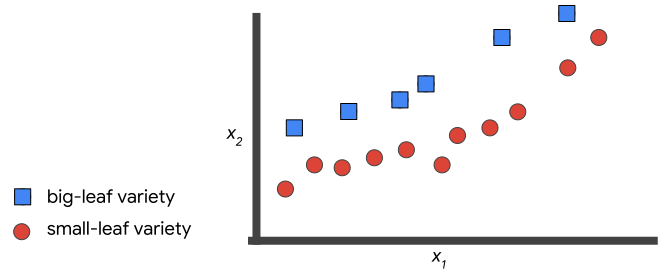
\includegraphics[width=\textwidth]{images/Graph1.png}

\end{frame}

%%

\begin{frame}{Supervised Learning}

\begin{itemize}
\item In supervised machine learning, you feed the features and their corresponding labels into an algorithm in a process called training. 

\item During training, the algorithm gradually determines the relationship between features and their corresponding labels. This relationship is called the model. 

\item Often times in machine learning, the model is very complex. 

\end{itemize}

\end{frame}

\begin{frame}{Supervised Learning}

\begin{itemize}

\item However, suppose that this model can be represented as a line that separates big-leaf from small-leaf:

\end{itemize}

\bigskip

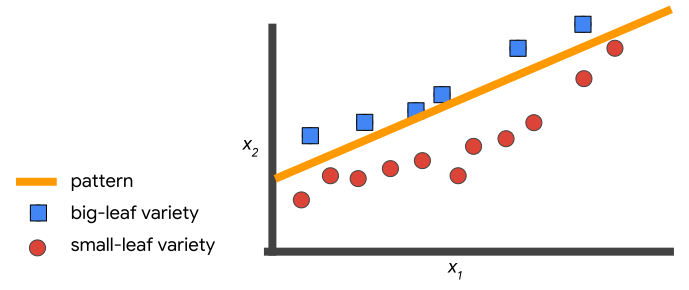
\includegraphics[width=\textwidth]{images/Graph2.png}

\end{frame}

%%%

\begin{frame}{Supervised Learning}

\begin{itemize}
\item Now that a model exists, you can use that model to classify new plants that you find in the jungle. For example:
\end{itemize}

\bigskip

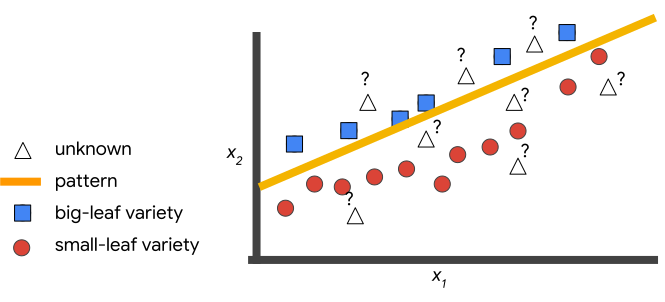
\includegraphics[width=\textwidth]{images/Graph3.png}

\end{frame}

%%%

\begin{frame}{Supervised Learning}

\begin{itemize}
\item To tie it all together, supervised machine learning finds patterns between data and labels that can be expressed mathematically as functions. 

\item Given an input feature, you are telling the system what the expected output label is, thus you are supervising the training. The ML system will learn patterns on this labeled data. 

\item In the future, the ML system will use these patterns to make predictions on data that it did not see during training.

\end{itemize}

\end{frame}

%%%

%\begin{frame}{Supervised Learning}
%
%\begin{itemize}
%
%\item A real-world example of supervised learning is a study from Stanford University that used a model to detect skin cancer in images. 
%
%\medskip
%\url{https://news.stanford.edu/2017/01/25/artificial-intelligence-used-identify-skin-cancer/}
%
%\item In this case, the training set contained images of skin labeled by dermatologists as having one of several diseases. 
%
%\item The ML system found signals that indicate each disease from its training set, and used those signals to make predictions on new, unlabeled images.
%
%\end{itemize}
%
%\end{frame}

%%%

\subsection{Unsupervised learning}

\begin{frame}{Unsupervised Learning}

\begin{itemize}

\item In unsupervised learning, the goal is to identify meaningful patterns in the data. 

\item To accomplish this, the machine must learn from an unlabeled data set. 

\item In other words, the model has no hints how to categorize each piece of data and must infer its own rules for doing so.

\end{itemize}

\end{frame}

%%%

\begin{frame}{Unsupervised Learning}

\begin{itemize}
\item All the examples are the same shape because we don't have labels to differentiate between examples of one type or another here:
\end{itemize}

\medskip

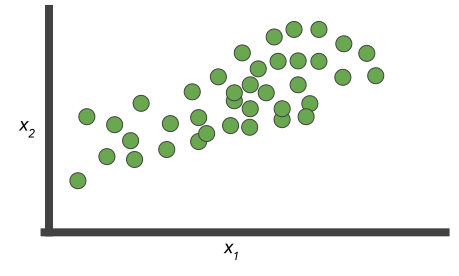
\includegraphics[width=0.8\textwidth]{images/Graph4.png}

\end{frame}

%%%

\begin{frame}{Unsupervised Learning}

\begin{itemize}
\item Fitting a line to unlabeled points isn't helpful. We still end up with examples of the same shape on both sides of the line. 
\end{itemize}

\includegraphics[width=0.8\textwidth]{images/Graph5.png}

\end{frame}

%%%

\begin{frame}{Unsupervised Learning}

\begin{itemize}
\item Here, we have two clusters. What do these clusters represent? It can be difficult to say. 

\end{itemize}

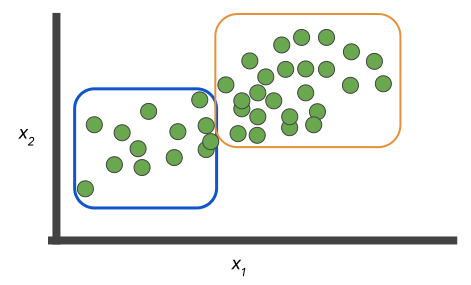
\includegraphics[width=0.8\textwidth]{images/Graph6.png}

\end{frame}

%%%

\begin{frame}{Unsupervised Learning}

\begin{itemize}
\item However, when new data arrives, we can categorize it pretty easily, assuming it fits into a known cluster. 

\end{itemize}

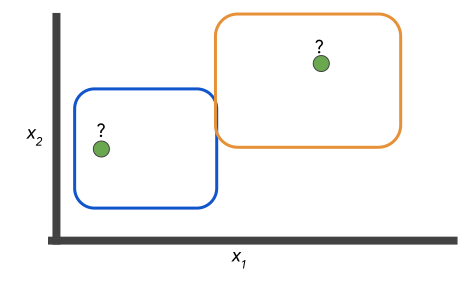
\includegraphics[width=0.8\textwidth]{images/Graph7.png}

\end{frame}

%%%

%\begin{frame}{Unsupervised Learning}

%\begin{itemize}
%\item But what if your photo clustering model has never seen a pangolin before? 

%\url{https://en.wikipedia.org/wiki/Pangolin}

%\item Will the system cluster the new photo with armadillos or maybe hedgehogs? 

%\url{https://en.wikipedia.org/wiki/Armadillo}

%\url{https://en.wikipedia.org/wiki/Hedgehog}
%\end{itemize}

%\end{frame}

%%%

\subsection{Reinforcement learning}

\begin{frame}{Reinforcement Learning}

\begin{itemize}
\item An additional branch of machine learning is reinforcement learning (RL). 

\item In RL you don't collect examples with labels. 

\item Imagine you want to teach a machine to play a very basic video game and never lose. 

\item You set up the model (often called an agent in RL) with the game, and you tell the model not to get a ``game over'' screen. 
\end{itemize}
\end{frame}

\begin{frame}{Reinforcement Learning}

\begin{itemize}

\item At time step $t$, the agent is in state $s_t$, takes action $a_t$, receives reward $r_t$, and transitions into state $s_{t+1}$.

\bigskip
\includegraphics[width=0.75\textwidth]{images/rl_diagram_transparent_bg.png}
\end{itemize}
\end{frame}

%%%

\begin{frame}{Reinforcement Learning}

\begin{itemize}
\item The state $s_t$ describes the agent's knowledge of the world. 

\item For instance, the visual input from a camera and the positions of the joints of a robot.

\item The agent has to learn which actions to take so as to maximize the total reward.  

\item For instance, a robot has to learn how to grasp and manipulate an object as fast as possible.
\end{itemize}

\end{frame}

%%%

%\begin{frame}{Reinforcement Learning}

%Look at the videos at \url{https://spinningup.openai.com/en/latest/spinningup/rl\_intro.html}

%\end{frame}

\begin{frame}{Reinforcement Learning}

\begin{itemize} 
\item You also need to provide a way for the agent to interact with the game to produce data.

\item This means either building a physical agent that can interact with the real world or a virtual agent and a virtual world, either of which is a big challenge. 

\end{itemize}

\end{frame}

%%%

\begin{frame}{Reinforcement Learning}

\url{https://gym.openai.com/}

\url{https://unity3d.com/machine-learning}

\url{https://openai.com/blog/openai-five/}

{\tiny
\url{https://deepmind.com/blog/article/AlphaStar-Grandmaster-level-in-StarCraft-II-using-multi-agent-reinforcement-learning}
}

\url{https://openai.com/blog/emergent-tool-use/}

\end{frame}

\end{document}

